\newcommand{\svcourse}{CST Part IA: Software Engineering and Security}
\newcommand{\svnumber}{1}
\newcommand{\svvenue}{Microsoft Teams}
\newcommand{\svdate}{2022-05-11}
\newcommand{\svtime}{15:00}
\newcommand{\svuploadkey}{CBd13xmL7PC1zqhNIoLdTiYUBnxZhzRAtJxv/ytRdM1r7qIfwMsxeVwM/pPcIo8l}

\newcommand{\svrname}{Dr Sam Ainsworth}
\newcommand{\jkfside}{oneside}
\newcommand{\jkfhanded}{yes}

\newcommand{\studentname}{Harry Langford}
\newcommand{\studentemail}{hjel2@cam.ac.uk}


\documentclass[10pt,\jkfside,a4paper]{article}

\usepackage[nocrest]{../../template/supervision}

\begin{document}

\section*{Questions}

\begin{enumerate}

    \item Consider two discrete probability distributions $p(x)$ and $q(x)$ over the same set of four values $\{x\}$ of a random variable:

    \begin{table}[H]

        \centering

        \begin{tabular}{c||c|c|c|c}
        $p(x)$ & $1/8$ & $1/8$ & $1/4$ & $1/2$ \\
        \hline
        $p(x)$ & $1/4$ & $1/4$ & $1/4$ & $1/4$ \\
        \end{tabular}

    \end{table}

    \begin{enumerate}

        \item Calculate the cross-entropy $H(p, q)$ between $p(x)$ and $q(x)$.
        \begin{align*}
            H(p, q)
            &= \sum_x p(x) \cdot \lg \frac1{q(x)} \\
            &= \frac18 \cdot \lg 4 + \frac18 \cdot \lg 4 + \frac14 \cdot \lg 4 + \frac12 \cdot \lg 4 \\
            &= \frac14 \lg 2 + \frac14 \lg 2 + \frac12 \lg 2 + \lg 2 \\
            &= 2\lg 2
        \end{align*}

        \item Calculate their Kullback-Leibler divergence $D_{\mathrm{KL}}(p \parallel q)$
        \begin{align*}
            D_{\mathrm{KL}}(p \parallel q)
            &= H(p, q) - H(p) \\
            &= 2\lg 2 - \sum_x p(x) \cdot \lg \frac{1}{p(x)} \\
            &= 2\lg 2 - \frac18 \lg 8 - \frac18 \lg 8 - \frac14 \lg 4 - \frac12 \lg 2 \\
            &= 2\lg 2 - \frac38 \lg 2 - \frac38 \lg 2 - \frac12 \lg 2 - \frac12 \lg 2 \\
            &= \frac14 \lg 2
        \end{align*}

        \item Comment on the use of the metrics $H(p, q)$ and $D_{\mathrm{KL}}(p \parallel q)$ in machine learning and for calculating the efficiency of codes.

        $H(p, q)$ is the metric often minimised in classification tasks. In this context $p$ would be the true probabilities (or class) and $q$ would be the predicted probabilities.

        $D_{\mathrm{KL}}(p \parallel q)$ is often maximised in the context of generative AI -- for example in Autoencoders, where the model learns to minimise the KL-divergence between the latent space representation of images encoded and the standard multivariate normal distribution. KL-divergence also occurs as a loss function in other ML disciplines -- such as Bayesian ML.

    \end{enumerate}

    \item Continuous random variables $X$ and $Y$ both have uniform probability density distributions on some interval. For $X$, $p(x) = 1/2$ if $x \in [0, 2]$, otherwise $0$, while for $Y$, $p(y) = 1/8$ if $y \in [0, 8]$, otherwise $0$. Calculate the differential entropies $h(X)$ and $h(Y)$.
    \begin{align*}
        h(X)
        &= \int^2_0 p(x) \cdot \ln \frac1{p(x)} \mathrm{d}x \\
        &= \int^2_0 \frac12 \cdot \ln \frac12 \mathrm{d}x \\
        &= \left[x \cdot \frac12 \cdot \ln 2 \right]^2_0 \\
        &= \ln 2
    \end{align*}
    \begin{align*}
        h(Y)
        &= \int^8_0 p(y) \cdot \ln \frac{1}{p(y)} \mathrm{d}x \\
        &= \int^8_0 \frac38 \cdot \ln 2 \mathrm{d}x \\
        &= \left[x \cdot \frac38 \cdot \ln 2 \right]^8_0 \\
        &= 3\cdot \ln 2
    \end{align*}

    \item

    \begin{enumerate}

        \item Find the optimal input distribution for the Binary Symmetric Channel and show that its capacity is given by $C = 1 - H_2(f)$.

        The optimal input distribution for the Binary Symmetric Channel is the distribution which maximises the mutual information $I(X; Y)$ between the output and the input. We can find this by differentiating the expression for the mutual information $I(X; Y)$ with respect to $p$.

        \begin{align*}
            I(X; Y)
            &= H(X) - H(X \mid Y) \\
            &= H_2(X) - H_2(f) \\
            \frac{\partial I(X; Y)}{\partial p}
            &= \frac{\partial H_2(X)}{\partial p}
        \end{align*}

        Thus, the optimal input distribution is that which maximises the entropy of the input. We know that entropy is maximised when events are equiprobable. Thus, the optimal input distribution occurs when $p = 1 - p = \frac12$.

        Substituting this back into the original expression gives:
        \[
            C = \max_p I(X; Y) = \max_p H_2(p) - H_2(f) = \frac12 \lg 2 + \frac12 \lg 2 - H_2(f) = 1 - H_2(f)
        \]

        \item Consider the $Z$ channel:)
        \begin{align*}
            P(y = 0 \mid x = 0) = 1 \\
            P(y = 1 \mid x = 0) = 0 \\
            P(y = 0 \mid x = 1) = f \\
            P(y = 1 \mid x = 1) = 1 - f \\
        \end{align*}

        Show that the mutual information given by ($p_1$ is $P(X = 1)$ for source $X$):
        \[
            I(X; Y) = H_2(p_1 (1 - f)) - p_1 H_2(f)
        \]

        \begin{align*}
            H(Y \mid X)
            &= \sum_x p(x) \sum_y h(p(y \mid x)) \\
            &= p_1 \cdot (h(f) + h(1 - f)) + p_2 \cdot (h(1) + h(0)) \\
            &= p_1 H_2(f) + p_2 0 \\
            &= p_1 H_2(f)
        \end{align*}

        \begin{align*}
            H(Y)
            &= \sum_y p(y) \lg \frac{1}{p(y)} \\
            &= \sum_y \sum_x p(x, y) \lg \frac{1}{\sum_x p(x, y)} \\
            &= (p_1 f + 1 - p_1) \lg \frac{1}{p_1 f + 1 - p_1} + (p_1(1 - f))\lg \frac{1}{p_1(1 - f)} \\
            &= (1 - p_1(1 - f)) \lg \frac{1}{1 - p_1(1 - f)} + (p_1(1 - f))\lg \frac{1}{p_1(1 - f)} \\
            &= H_2(p_1(1 - f))
        \end{align*}

        \begin{align*}
            I(X; Y)
            &= H(Y) - H(Y \mid X) \\
            &= H_2(p_1 (1 - f)) - p_1 H_2(f)
        \end{align*}

        Hence show that the optimal input distribution is given by
        \[
            p_1^\star = \frac{1/(1 - f)}{1 + 2^{H_2(f)/(1 - f)}}
        \]

        We can find the optimal input distribution by differentiating the mutual information with respect to $p_1$ and finding the maxima.

        \begin{align*}
            I(X; Y)
            &= H_2(p_1 (1 - f)) - p_1 H_2(f) \\
            \frac{\partial I(X; Y)}{\partial p_1}
            &= \frac{\partial}{\partial p_1 (1 - f)}(H_2(p_1 (1 - f))) \cdot \frac{\partial}{\partial p_1}(p_1 (1 - f)) - H_2(f) \\
            &= - \lg \frac{p_1(1 - f)}{1 - p_1(1 - f)} \cdot (1 - f) - H_2(f) \\
            0 &= - (1 - f) \lg \frac{p_1^\star(1 - f)}{1 - p_1^\star(1 - f)} - H_2(f) \\
            2^{\frac{H_2(f)}{1 - f}} &= \frac{1 - p_1^\star(1 - f)}{p_1^\star(1 - f)} \\
            p_1^\star(1 - f) &= \frac{1}{1 + 2^{\frac{H_2(f)}{1 - f}}} \\
            p_1^\star &= \frac{1/(1 - f)}{1 + 2^{H_2(f)/(1 - f)}}
        \end{align*}

        \item Plot a graph of $p_1^*$ and investigate what happens as the noise level $f$ becomes close to $1$. Observe that $p_1^* < 0.5$, for all values of $f$.

        \begin{figure}[H]

            \centering

            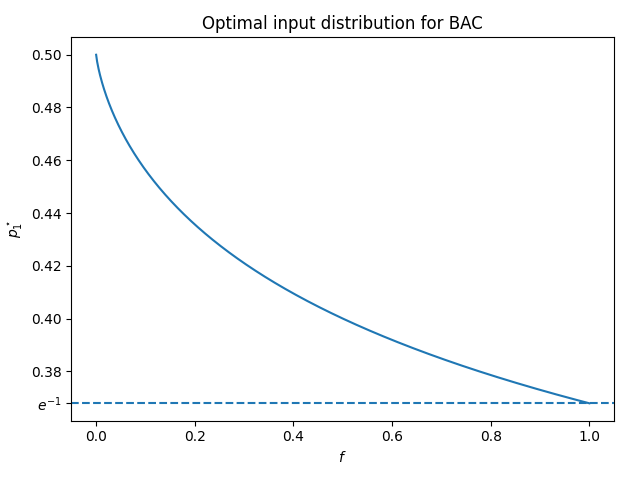
\includegraphics[width=0.6\textwidth]{bac-plot}

            \caption{A graph of the optimal input distribution $p^\star_1$ of a BAC against the error probability}

        \end{figure}

        Notice that $\lim_{f \to 1} p_1^\star = e^{-1}$.

        \item Sketch graphs of the capacity of the binary symmetric channel and the $Z$ channel as a function of $f$.

        \begin{figure}[H]

            \centering

            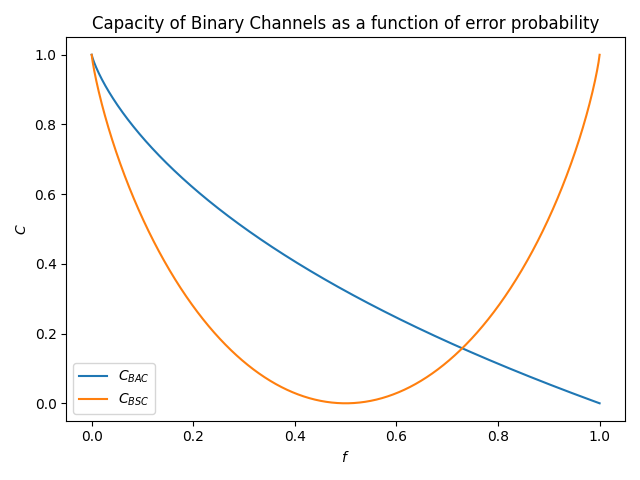
\includegraphics[width=0.6\textwidth]{bsc-bac-capacity}

            \caption{A graph of the capacity of BSC's and BAC's against the error probability}

        \end{figure}

    \end{enumerate}

    \item A continuous communication channel adds Gaussian white noise to signals transmitted through it. The ratio of signal power to noise power is 30 decibels, and the frequency bandwidth of this channel is 10MHz. roughly what is the information capacity $C$ of this channel, in bits/second?
    \begin{align*}
        C
        &= B \cdot \lg \left( 1 + \frac{S}{N} \right) \\
        &= 10\times 10^6 \cdot \lg \left( 1 + 30 \right) \\
        &= 49.5\ldots \times 10^6
    \end{align*}

    \item

    \begin{enumerate}

        \item In lectures, you have seen correlation.  related concept, the autocorrelation of a signal (correlation of a signal with itself after some time lag) is defined as
        \[
            R_{yy}(\ell) = \sum_{n \in \mathbb Z} y(n) \overline{y(n - \ell)}
        \]
        The following CSV file contains a sine wave $(\sin(2\pi f_0 t_i))$ embedded in additivee white Gaussian Noise: \url{http://ireland.cx/teaching/2122/infoth/autocorrelation.txt}. The sampling frequency is 2 MHz.

        Plot the autocorrelation of the signal in the CSV file ($R_{yy}(\ell)$ against $\ell$). Hence find the frequency $f_0$ of the sine wave.

        \begin{figure}[H]

            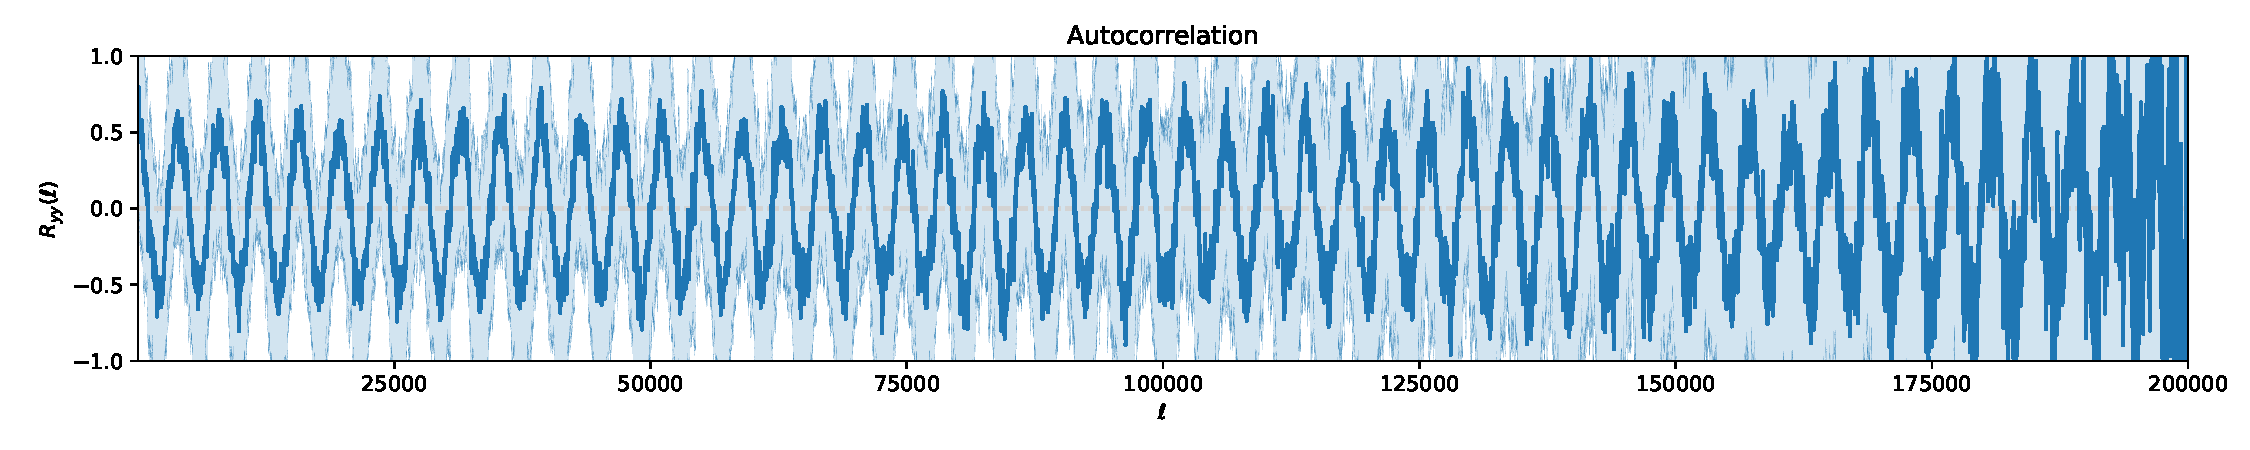
\includegraphics[width=\textwidth]{./autocorelation.pdf}

            \caption{Graph of $\ell$ against $R_{yy}(\ell)$}

            \label{fig:sinewave}

        \end{figure}

        As we see in~\cref{fig:sinewave}, the autocorrelation mirrors a wave. When $\ell$ is close to the true offset, we have that the autocorrelation is high. When it is half the period, we have low autocorrelation.

        Note that the true autocorrelation was too noisy. So, I plot the mean over 50 adjacent values on either side (and \texttt{fill\_between} standard deviation). From this. Observe that the autocorrelation ``cycles'' every 4000 readings. This implies that the frequency of the sine wave $f_0$ is roughly $\frac{1}{4000} \cdot 2000000 \approx 500Hz$.

        \item Research and explain how GPS works at the physical and data-link layers. Explain how GPS implements the spreading of the spectrum of the transmitted signal over a very large bandwidth, and how the wide-bandwidth signal is decoded in a GPS receiver.

        \todo{Do this!}

    \end{enumerate}

    \item Explain the concept of entropy in:

    \begin{enumerate}

        \item Classical thermodynamics (``entropy'', developed by Clausius and others)

        Classical Entropy is a measure of disorder and represents the energy of a system which is \emph{not} available for work.

        \item Statistical mechanics (``statistical entropy'', developed by Boltzmann and others -- presented in lecture 12)

        A measure of the number of possible states that a system in thermodynamic equilibrium could be in.

        \item Information theeory (``information entropy'', developed by Shannon)

        The average amound of information required to completely describe a state.

    \end{enumerate}

    To what extent do these different notions of entropy relate to each other?

    These notions of entropy are similar at an intuitive level. They are all measures of how much we \emph{don't} know about a state. This means they're \emph{related}.

\end{enumerate}

\end{document}
